\documentclass[14pt,a4paper]{article} %openany
\usepackage[affil-it]{authblk}
\usepackage[english]{babel}
\usepackage{graphicx}
\usepackage{rotating}
%\usepackage{bibtex}
%\usepackage[utf8]{inputenc}
%\usepackage[english]{babel}
\usepackage{adjustbox}
\usepackage{courier}
\usepackage{verbatim}
\usepackage{url}
\usepackage[hidelinks]{hyperref}
\usepackage{float}
\usepackage{array}
\usepackage{breakcites}
\usepackage{gensymb}
%\usepackage[backend=biber]{biblatex}
\usepackage{booktabs,tabularx}
\usepackage{listings}
\usepackage{appendix}
\usepackage{cite}
\usepackage{blindtext}
\usepackage[utf8]{inputenc} % Required for inputting international characters
\usepackage[T1]{fontenc} % Output font encoding for international characters
\usepackage{mathpazo} % Palatino font
\usepackage{graphicx} % For the logo
\usepackage[acronym,toc]{glossaries}
\newacronym{<++>}{<++>}{<++>}
\newacronym{I$^2$CNER}{I$^2$CNER}{International Institute for Carbon Neutral Energy Research}
\newacronym{MARKAL}{MARKAL}{MARKet ALlocation}
\newacronym{TIMES}{TIMES}{The Integrated MARKAL-EFOM System}
%\newacronym[longplural={metric tons of heavy metal}]{MTHM}{MTHM}{metric ton of heavy metal}


\usepackage{amssymb}
\usepackage{pifont}
\usepackage{ragged2e}
\usepackage{xcolor}
\newcommand{\greencheck}{{\color{green}\checkmark}}
\newcommand{\xmark}{{\color{red}\ding{55}}}

%\bibliographystyle{numeric}

\begin{document}

%----------------------------------------------------------------------------------------
%    TITLE PAGE
%----------------------------------------------------------------------------------------

\begin{titlepage} % Suppresses displaying the page number on the title page and the subsequent page counts as page 1
    \newcommand{\HRule}{\rule{\linewidth}{0.5mm}} % Defines a new command for horizontal lines, change thickness here
    
    \center % Centre everything on the page

    %------------------------------------------------
    %    Title
    %------------------------------------------------
    
    \HRule\\[0.2cm]
    
     \begin{minipage}{0.4\textwidth}
        
\includegraphics[width=\textwidth]{arfc-logo}
        \end{minipage}%
        \begin{minipage}{0.6\textwidth}
        {\begin{flushright}\huge\bfseries Dynamic Transition Analysis With \gls{TIMES} \end{flushright}}
        {\begin{flushright}\large\textit{\gls{I2CNER} Project Report}\end{flushright}}

        \end{minipage}

    \vspace{0.2cm}
    \HRule
    \vspace{0.5cm}
    
    %------------------------------------------------
    %    Author(s)
    %------------------------------------------------
    
    \begin{minipage}{0.4\textwidth}
        \begin{flushleft}
            \large
            \textit{Author}\\
            Anshuman \textsc{Chaube}\\
        \end{flushleft}
    \end{minipage}
    ~
    \begin{minipage}{0.4\textwidth}
        \begin{flushright}
            \large
            \textit{Principal Investigator}\\
            Kathryn D. \textsc{Huff} % Supervisor's name
            \vspace{4mm}\\
            \textit{Co-Principal Investigator}\\
            James \textsc{Stubbins} % Supervisor's name
            \vspace{4mm}\\
            \textit{Contributing Collaborators}\\
            Kenshi \textsc{Itaoka} \\% Supervisor's name
            Andrew \textsc{Chapman} \\% Supervisor's name
            Hadi \textsc{Faradi} \\% Supervisor's name
        \end{flushright}
    \end{minipage}
    
    % If you don't want a supervisor, uncomment the two lines below and comment the code above
    %{\large\textit{Author}}\\
    %John \textsc{Smith} % Your name

    %------------------------------------------------
    %    Report Number
    %------------------------------------------------
    \vspace{1cm}
    \textsc{\LARGE\bfseries UIUC-ARFC-2019-02} % Replace YYYY with the year, NN with report index
    \vspace{0.5cm}
    
    %------------------------------------------------
    %    Date
    %------------------------------------------------
    
    \vspace{0.5cm} % Position the date further down the remaining page
    {\large May 29, 2019} % Date, change the \today to a set date if you want to be precise
    \vspace{0.5cm}

%------------------------------------------------
    %    Headings
    %------------------------------------------------
    
    \textsc{\LARGE Advanced Reactors and Fuel Cycles}\\[0.25cm] % Research Group
    
    \textsc{\large Dept. of Nuclear, Plasma, \& Radiological Engineering}\\% Department
    
    \textsc{\large University of Illiois at Urbana-Champaign}\\ % University


    
    %------------------------------------------------
    %    Logo
    %------------------------------------------------
    
    
    \vspace{0.5cm}
    
\includegraphics[scale=0.2]{arfc-smol}
    
\includegraphics[scale=0.3]{i2cner-logo}
    
\includegraphics[scale=0.2]{wpi-logo}
    
\includegraphics[scale=0.04]{ku-logo}\\[1cm] % Include a department/university logo - this will require the graphicx package
     
    %----------------------------------------------------------------------------------------

    %------------------------------------------------
    %   Funding 
    %------------------------------------------------
    % For this section, either use \vfill to fill the space 
    % or insert funding acknowledgement
    \textit{The authors gratefully acknowledge the support of the International Institute for Carbon
Neutral Energy Research (WPI-I2CNER), sponsored by the Japanese Ministry of Education, Culture, Sports, Science and Technology.}  

\end{titlepage}

\section{Introduction}
We initiated a project in January 2018 to simulate dynamic transition scenarios for the energy industry in Japan to suggest pathways for minimizing carbon emissions. This report is a summary of the progress we have made so far, the challenges we currently face, and the future direction of this research. 

\section{Progress Summary}

The tasks that we performed can be divided into two categories: technical tasks associated with implementation of details and features in our model, and data collection and organization. Our accomplishments have been:

\subsection{Installation of and familiarization with VEDA (January – March 2018)}
To model Japan's energy industry, we chose VEDA, a \gls{TIMES} \cite{loulou_documentation_2005,gargiulo_documentation_2005} shell. Using the simplest VEDA input files from the VEDA tutorial \cite{gargiulo_documentation_2005} as a starting point, we developed our own model files, which we have been progressively refining since then.

At the same time, we collected data pertaining to electricity generation and carbon emissions.

\subsection{Incorporation of fossil fuel-related data(April – May 2018)}
We incorporated data for electricity generation from fossil fuels from the \gls{EDMC} databank\cite{noauthor_energy_2018}, along with creating a simplified demand process reflecting recent trends in electricity demand in Japan.\\

While collecting these data, we noticed that the \gls{EDMC} databank that we have been relying on has no data for the amount of electricity generated from individual fossil fuels for the years 2011-12. Instead, the amount of electricity generated from coal, oil, and natural gas is lumped together in one category entitled "thermal". Further, the 2016 data seem slightly inconsistent across different data tables in the \gls{EDMC} databank. The source of variation in these numbers is likely to be the changes in the electricity distribution system of Japan since 2016.

\subsection{Incorporation of nuclear, hydropower and renewables into the model(June – August 2018)}
The process of incorporating these into the model was similar to that for previously mentioned energy sources but simpler, since the data obtained for these energy sources from \gls{EDMC} were consistent across \gls{EDMC} data tables and secondary sources \cite{noauthor_energy_2018,noauthor_iea_2017, noauthor_japan_2017}. We have also included processes for the projected growth of nuclear, solar and wind based on data from various studies, reports and articles. \cite{publicover_japan_2017, dincer_analysis_2011,noauthor_geothermal_2018,heger_wind_2016,noauthor_operational_2013,noauthor_electricity_2017}

\subsection{Refining CO\textsubscript{2} emission processes(August – September 2018)}
While we had been modelling CO\textsubscript{2} emission processes in parallel with the electricity generation processes, it was only after incorporating all conventional energy sources that we could move on to aligning the model's CO\textsubscript{2} emission values with actual emissions from Japan. The major obstacle we faced was the absence of data pertaining to electricity generation from individual fossil fuels, with each fossil fuel's energy cycle having different emission coefficients. We estimated the missing figures based on previous years' trends \cite{noauthor_energy_2018,noauthor_national_2018} and obtained reasonable approximations of electricity generation (see fig. \ref{elcic}), which result in CO\textsubscript{2} emission values that differ from actual values by about 5\% at most (see fig. \ref{co2ic} and \ref{co2err}).\\

\subsection{October 2018 – January 2019}

\subsubsection{Changing simulation timeframe to 2013-2100}
As discussed previously, it became impossible to find exact data for fossil fuels for the years 2010,2011 and 2012. Hence the total CO$_2$ emissions for those years were very slightly off the mark. We sidestepped this problem by changing the initial year to 2013, for which we have exact data from \gls{EDMC} \cite{noauthor_energy_2018}.

\subsubsection{Incorporation of the \gls{PEAK} factor \cite{gargiulo_documentation_2005} factor}
This parameter is defined as the fraction of a resource's installed capacity that is guaranteed to be available during peak demand. This introduces a notion of an energy resource's reliability. Its incorporation reduced excessive deployment of wind and solar. However, the \gls{PEAK} factor values in the model \cite{kato_energy_2016} neglect the daily or seasonal variation of wind and solar, as the factor is annually averaged.

\subsubsection{Basic \gls{CCS} Implementation}
Some \gls{CCS} data \cite{kato_energy_2016}  were incorporated into \href{https://github.com/arfc/i2cner/tree/master/JPN-Main-Model/active/i2cner-nonuc}{one of the models}. However, no \gls{CCS} gets deployed in our models. We believe  it should be deployed for an intermediate time-period, since in the absence of nuclear, only \gls{CCS} can provide reliable, clean energy in conjunction with renewables. We have identified a few shortcomings in our model, some of which contribute to this problem:

\paragraph{Large amounts of offshore wind can be deployed:} While we were initially reluctant to hard-code strict installed  capacity limits into our model, we have since realized that Japan's underdeveloped offshore wind industry will not reach its full potential for a very long time, as offshore wind is extremely expensive to deploy in Japan. This is due to the unusually deep seabed that is very close to the Japanese coast. \gls{JWPA} projections \cite{heger_wind_2016} are already ambitious, and our models should be closely aligned with them.

\paragraph{Wind and solar's daily and seasonal variance neglected:} Their capacity factor is annually averaged. Their installed capacity should be matched by electricity storage or natural gas. Possible ways to implement this are discussed later.

\paragraph{We may be overestimating \gls{CCS} costs:} The costs associated with \gls{CCS} for Japan have been hard to find as Japan, instead of building \gls{CCS} pipelines like the US or China, intends to build a shipping network for offshore storage of captured and compressed CO$_2$. While this would make \gls{CCS} plants more expensive in Japan, we cannot arrive at an exact figure. Based on our interaction with our Energy Analysis Division colleagues at Kyushu university, the costs of this are still being explored by the Japanese government.

\subsection{February 2019 – April 2019:}

\subsubsection{Gradual collection and replacement of \gls{LCOE} data with accurate cost structure}
The results presented at the \gls{I2CNER} Annual \gls{EAD} workshop \cite{chaube_dynamic_2019} were based entirely on \gls{LCOE} analysis, as \gls{LCOE} data and projections were readily available. However, it is more suitable to incorporate cost data in the recommended \gls{TIMES} format, that is with the investment/capital cost, and fixed and variable \gls{OM} costs. We believe that when there is no investment cost associated with an energy source, the deployment or premature retirement has no cost-penalty. This may cause resource deployments for unrealistically brief periods (see fig. \ref{flatgood}).

\subsubsection{Incorporation of semi-discrete investment sizes}
Discrete investment sizes were incorporated in most scenarios' \gls{DSCINV} files\cite{gargiulo_documentation_2005}, whereas the slightly improved semi-discrete installed  capacity sizes are incorporated in the \href{https://github.com/arfc/i2cner/tree/master/JPN-Main-Model/active/co2-constrnt-conv-nonuc}{conventional-no-nuclear model} (see Table \ref{tab:models}). It is desired that all \gls{DSCINV} files in the remaining three models include a similar semi-discrete installed  capacity installation structure, as this helps eliminate the production-exceeding-demand bug (see fig. \ref{flatbug} and fig. \ref{flatgood}).

\section{Model description}

The objective function \cite{loulou_documentation_2005} for the simulation is the system cost, and the primary constraints are the demand and the limit on CO$_2$ emissions based on \gls{I2CNER} goals. Hence, the simulations determine the energy mix most economically optimal for meeting Japan's future energy needs, when constrained by \gls{I2CNER} CO$_2$ emissions.

\subsection{Key Simulation Parameters}

The models include some combination of the technologies mentioned in Table \ref{tab:basic}; the exact combination for each model is described in Table \ref{tab:models}.

\begin{table}[H]
\centering
\caption{\label{tab:basic} Main simulation parameters and features.}
\begin{tabular}{|c|c|}
\hline
Start year & 2013 \\
\hline
End Year & 2100 \\
\hline
Demand increase rate & +1.7\% p.a. \cite{noauthor_electricity_2017} \\
\hline
Conventional sources & Coal, Oil, Natural Gas, Combined Cycle, Nuclear \\
\hline
Renewables & Solar, Wind, Geothermal, Hydro \\
\hline
Novel tech. & H$_2$(photocatalytic), \gls{CCS} (point-capture)\\
\hline
\end{tabular}
\end{table}

\begin{table}[H]
\centering
\caption{\label{tab:models} Model description.}
\begin{tabular}{| c | c | c | c |}
\hline
\textbf{Model Name}&\textbf{Conventional}&\textbf{Novel}&\textbf{New nuclear}\\
            &\textbf{technology}&\textbf{technology}&\textbf{reactors}\\
                  \hline
conv-free &      \greencheck           &         \xmark       &      \greencheck     \\ 
conv-nonuc &      \greencheck           &         \xmark       &         \xmark       \\ 
i2cner-free &      \greencheck           &      \greencheck     &      \greencheck     \\ 
i2cner-nonuc &      \greencheck           &      \greencheck     &         \xmark       \\
\hline
\end{tabular}
\end{table}

\subsection{Assumptions}

Our model focuses on the electricity generation sector. The following assumptions and limitations are present in our model:
	
\begin{enumerate}

\item All the energy generated by a given process is transferred to the grid without losses. Since the \gls{EDMC} data have units of electrical energy produced (GWh), we have no need of incorporating data about raw fossil fuel consumption, plant efficiency, and utilization factors for the initially deployed electricity generation sources.

\item \gls{LCOE} for fossil fuels and nuclear has been held constant throughout the simulation \cite{chapman_energy_2018,noauthor_lazards_2017,noauthor_iea_2017}. \gls{LCOE} projections for wind and solar have been incorporated \cite{noauthor_lazards_2017}.

\item Oil-based electricity is retired relatively quickly, and new oil-based electricity deployment is disabled, due to the emphasis of the Japanese government on energy self-sufficiency and minimizing costs, and due to a general trend in the \gls{EDMC} data \cite{noauthor_energy_2018} indicating declining use of oil.

\item Nuclear installed  capacity is increased in chunks equivalent to the installed  capacity of GE-Hitachi's \gls{ABWR} \cite{ge_advanced_2007}, which are under consideration for construction \cite{noauthor_electricity_2017}.

\item Solar – Any new solar installed  capacity created by the model has been assumed to be non-tracking type.

\item Hydropower – held constant at current levels.

\item Geothermal is expanded to its maximum potential \cite{noauthor_geothermal_2018}.

\item The CO\textsubscript{2} emission constraints implemented are representative of \gls{I2CNER} goals of an 80\% reduction in emissions from 1990 levels.
\end{enumerate}

\subsection{Model Data}

\textbf{Emission coefficients} \cite{noauthor_electricity_2017}: The emission coefficients are listed in Table \ref{tab:emi}. The data are in gCO$_2$/kWh. Hence, nuclear, solar and wind emissions from construction are averaged over the lifetime of the generation facility.

\begin{table}[H]
\centering
\caption{\label{tab:emi} List of emission coefficients used in the model.}
\vspace{2mm}
\begin{tabular}{|c|c|}
\hline
\textbf{Electricity source} & \textbf{Emissions coefficient}\\
\hline
Coal & 943 \\
\hline
Natural Gas & 599 \\
\hline
Oil & 738 \\
\hline
Solar & 38 \\
\hline
Wind & 25 \\
\hline
Nuclear & 21 \\
\hline
Geothermal & 13 \\
\hline
Hydropower & 11 \\
\hline
\end{tabular}
\end{table}

\textbf{\gls{LCOE}}\cite{noauthor_lazards_2017} : \gls{LCOE} data are appropriate for use in processes in which a fixed amount of installed capacity has already been deployed, i.e. the initial installed capacity, and where only the relative cost is important. The \gls{LCOE} data (in million USD/GWh) are listed in Table \ref{tab:lcoe}. \\

\begin{table}[H]
\centering
\caption{\label{tab:lcoe} \gls{LCOE} data used in the simulation.}
\vspace{2mm}
\begin{tabular}{|c|c|}
\hline
\textbf{Electricity source} & \textbf{LCOE}\\
\hline
Coal & 0.06 \\
\hline
Natural Gas & 0.08 \\
\hline
Oil & 0.39 \\
\hline
Solar & 0.161 \\
\hline
Wind & 0.144 \\
\hline
Nuclear & 0.1 \\
\hline
Geothermal & 0(fixed installed  capacity) \\
\hline
Hydropower & 0 (fixed installed  capacity) \\
\hline
\end{tabular}
\end{table}

\textbf{Detailed costs} \cite{noauthor_eia_2019} : While the models with conventional energy sources have part of the cost structure listed in Table \ref{tab:costs}, these somewhat inaccurate and highly idealized figures need to be revised based on the data in the \gls{ARFC} \gls{I2CNER} repository, especially for offshore and onshore wind(current data are for the US from the \gls{EIA} \cite{noauthor_eia_2019}), and for nuclear (to take construction delays into account).

\begin{table}[H]
\centering
\caption{\label{tab:costs} Detailed cost structure incorporated in some models.}
\vspace{2mm}
\begin{tabular}{|c|c|c|c|}
\hline
\textbf{Electricity} & \textbf{Investment} & \textbf{Fixed \gls{OM}} & \textbf{Variable \gls{OM}}\\
\textbf{source} & \textbf{Cost (MUSD/GWh)} & \textbf{Cost (MUSD/GW)} & \textbf{Cost (MUSD/GWh)}\\
\hline
Coal & 3784 & 51.39 & 0.0072\\
\hline
Combined Cycle & 794 & 10.3 & 0.0021\\
\hline
Solar & 1783 & 22.46 & 0 \\
\hline
Onshore Wind & 2773 & 40.85 & 0\\
\hline
Offshore Wind & 8380 & 80.14 & 0\\
\hline
Nuclear & 1600 & 0.0165 & 0.00933\\
\hline
\end{tabular}
\end{table}

\textbf{Miscellaneous VEDA Parameters} \cite{kato_energy_2016,gargiulo_documentation_2005}: The remaining TIMES parameters used in the models are listed in Table \ref{tab:misc}.
\begin{table}[H]
\centering
\caption{\label{tab:misc} Miscellaneous simulation parameters.}
\vspace{2mm}
\begin{tabular}{|c|c|c|c|c|}
\hline
\textbf{Electricity source} & \textbf{Efficiency} & \textbf{Utilization Factor} & \textbf{Lifetime (y)} & \textbf{\gls{PEAK} factor}\\
\hline
Coal & 0.6 & 0.95 & 60 & 1.0 \\
\hline
Combined Cycle & 0.5 & 0.95 & 60 & 1.0 \\
\hline
Solar & 0.20-0.27 & 0.13 & 20-25 & 0.42 \\
\hline
Onshore Wind & 0.9 & 0.23-0.25 & 25 & 0.20 \\
\hline
Offshore Wind & 0.9 & 0.31-0.32 & 25 & 0.20 \\
\hline
Nuclear & 0.9 & 0.95 & 60 & 1.0 \\
\hline
\end{tabular}
\end{table}

\section{Results}

Based on these assumptions and data(\gls{LCOE}), the model yields the following results for the years 2011-16 (see figure \ref{elcic}), which are within 5\% of the actual electricity generation figures obtained from \gls{EDMC}. \gls{LCOE}-based results for the entire time-period are present in the poster presented at the \gls{I2CNER} symposium \cite{chaube_dynamic_2019}.

\begin{figure}[H]
\centering
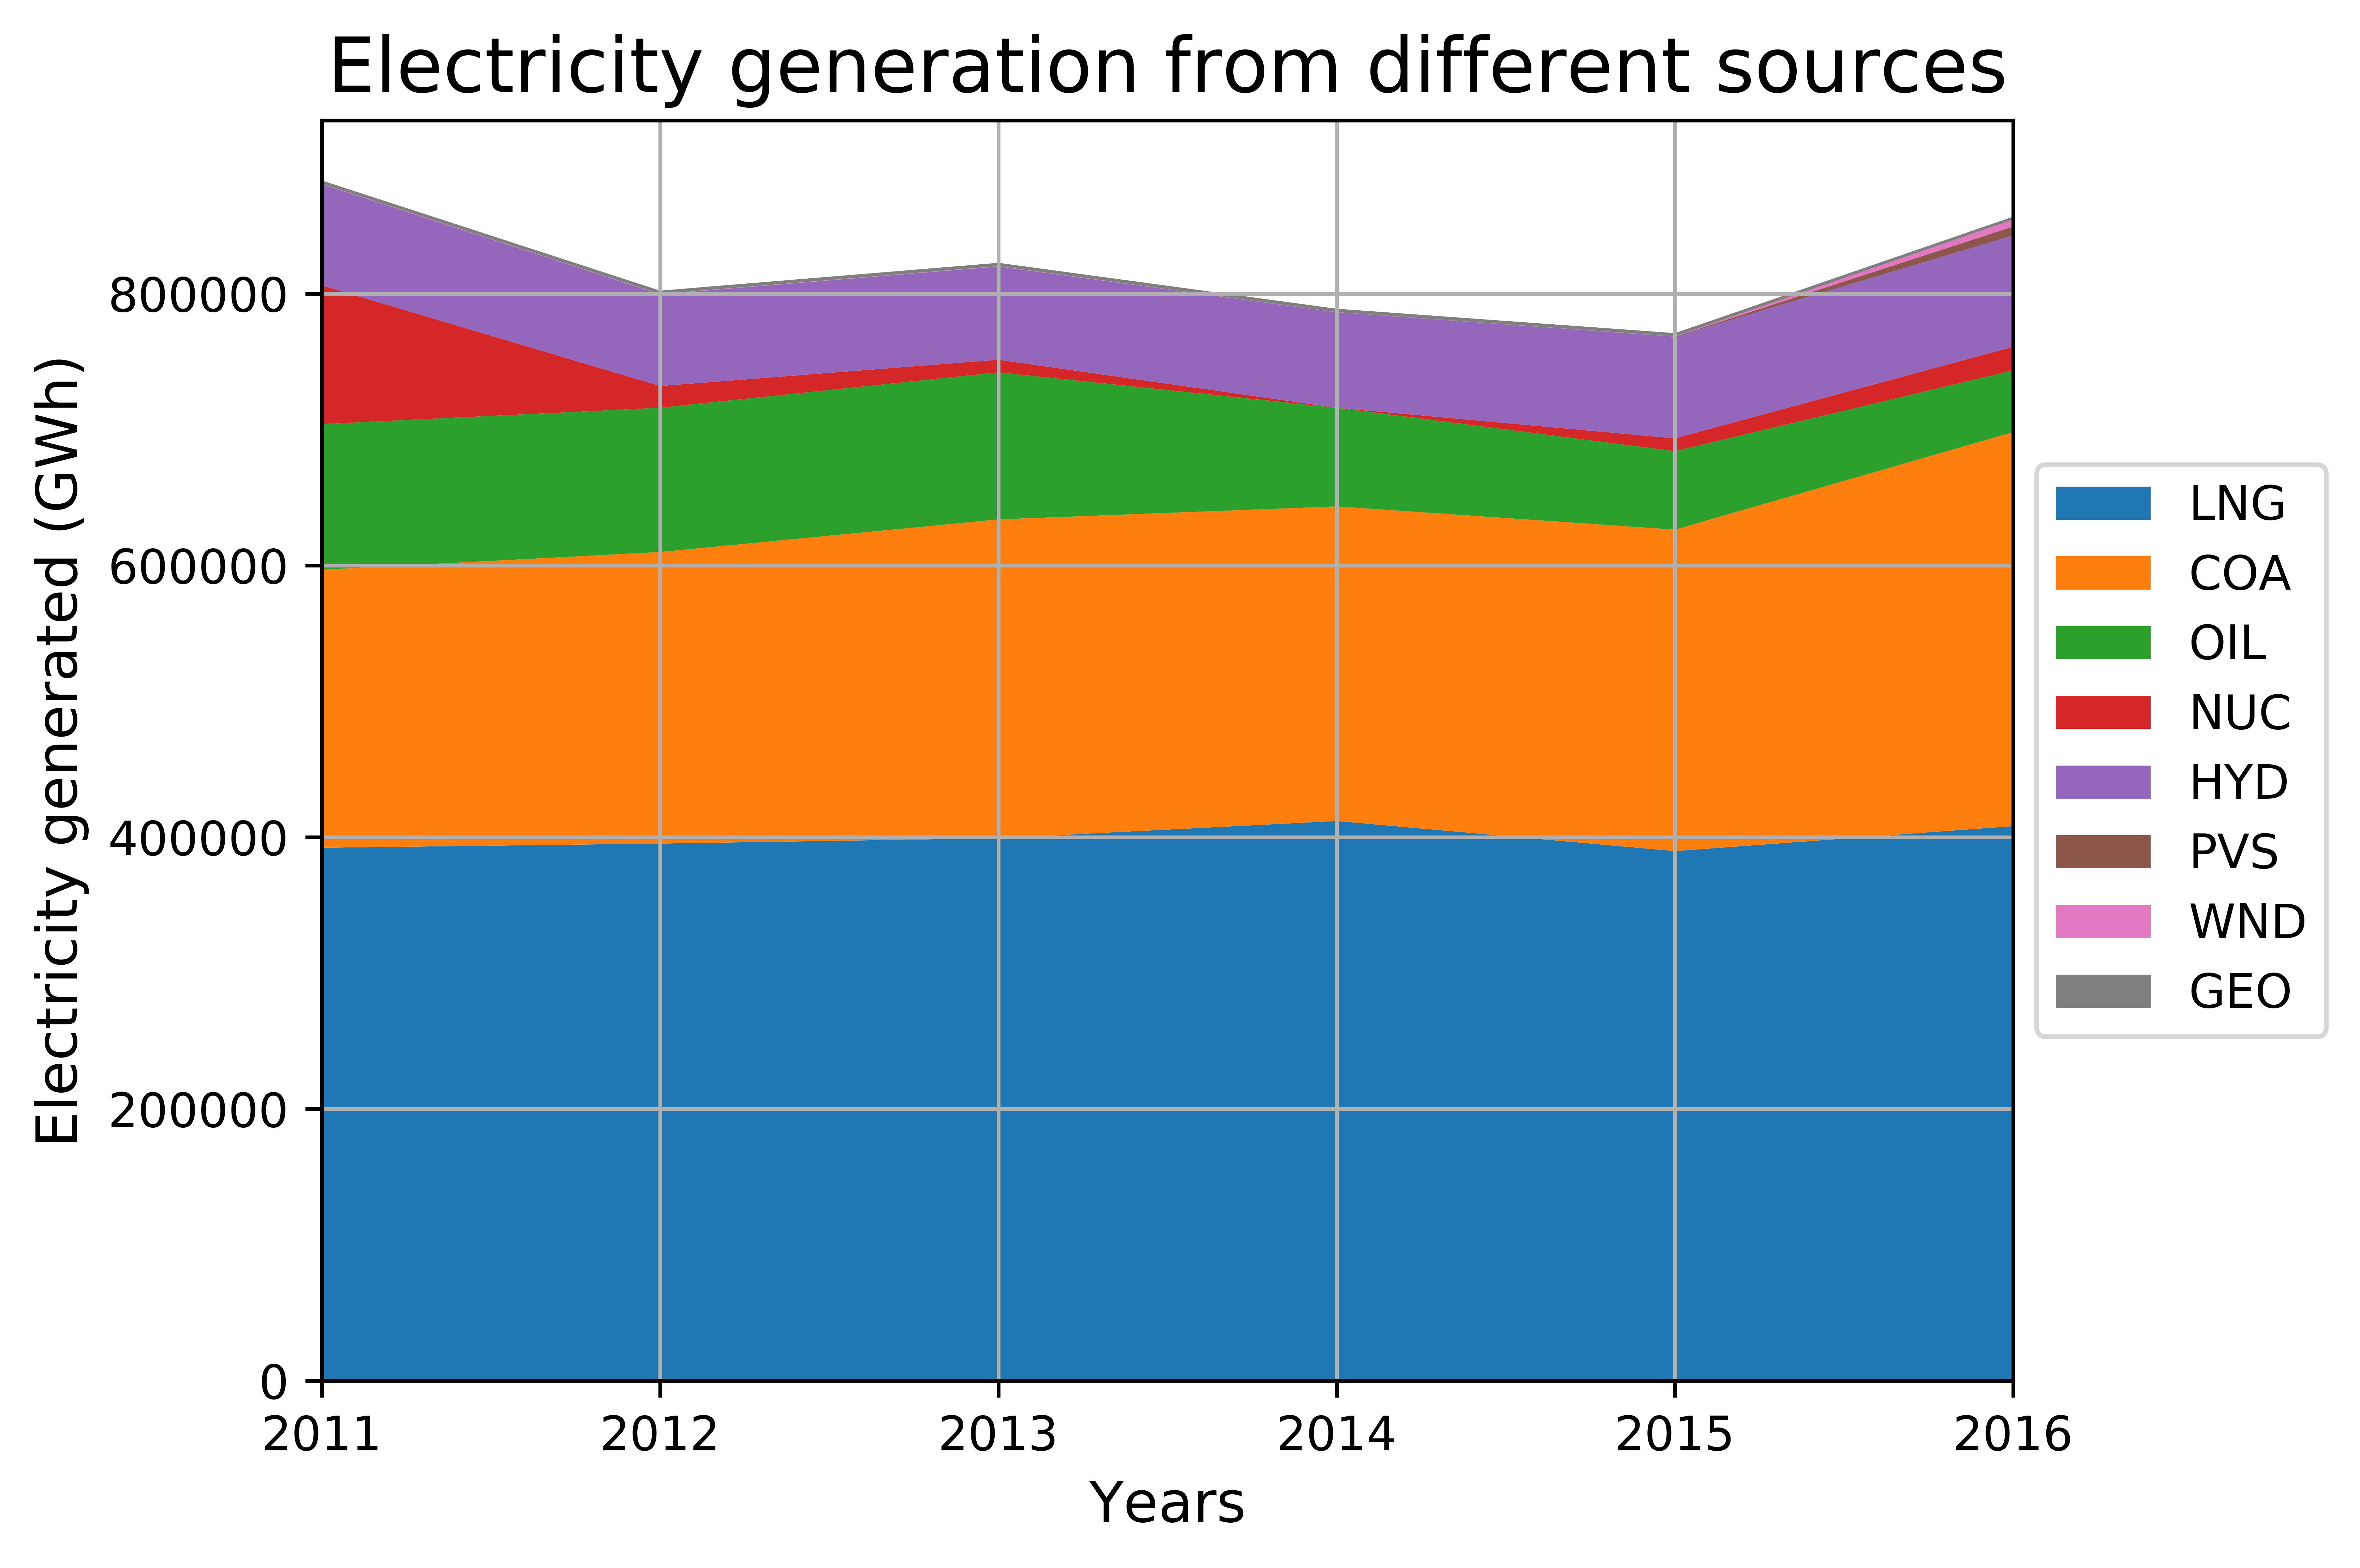
\includegraphics[scale=0.6]{elc-2016}
\caption{Electricity generation profile for the model's initial conditions.}
\label{elcic}
\end{figure}

The CO\textsubscript{2} emissions for the period 2011-16 are shown in figure \ref{co2ic}. The maximum error is 5.7\% (see figure \ref{co2err}), which is due to the aforementioned absence of accurate data for 2011, 2012 and 2016. 

\begin{figure}[H]
\centering
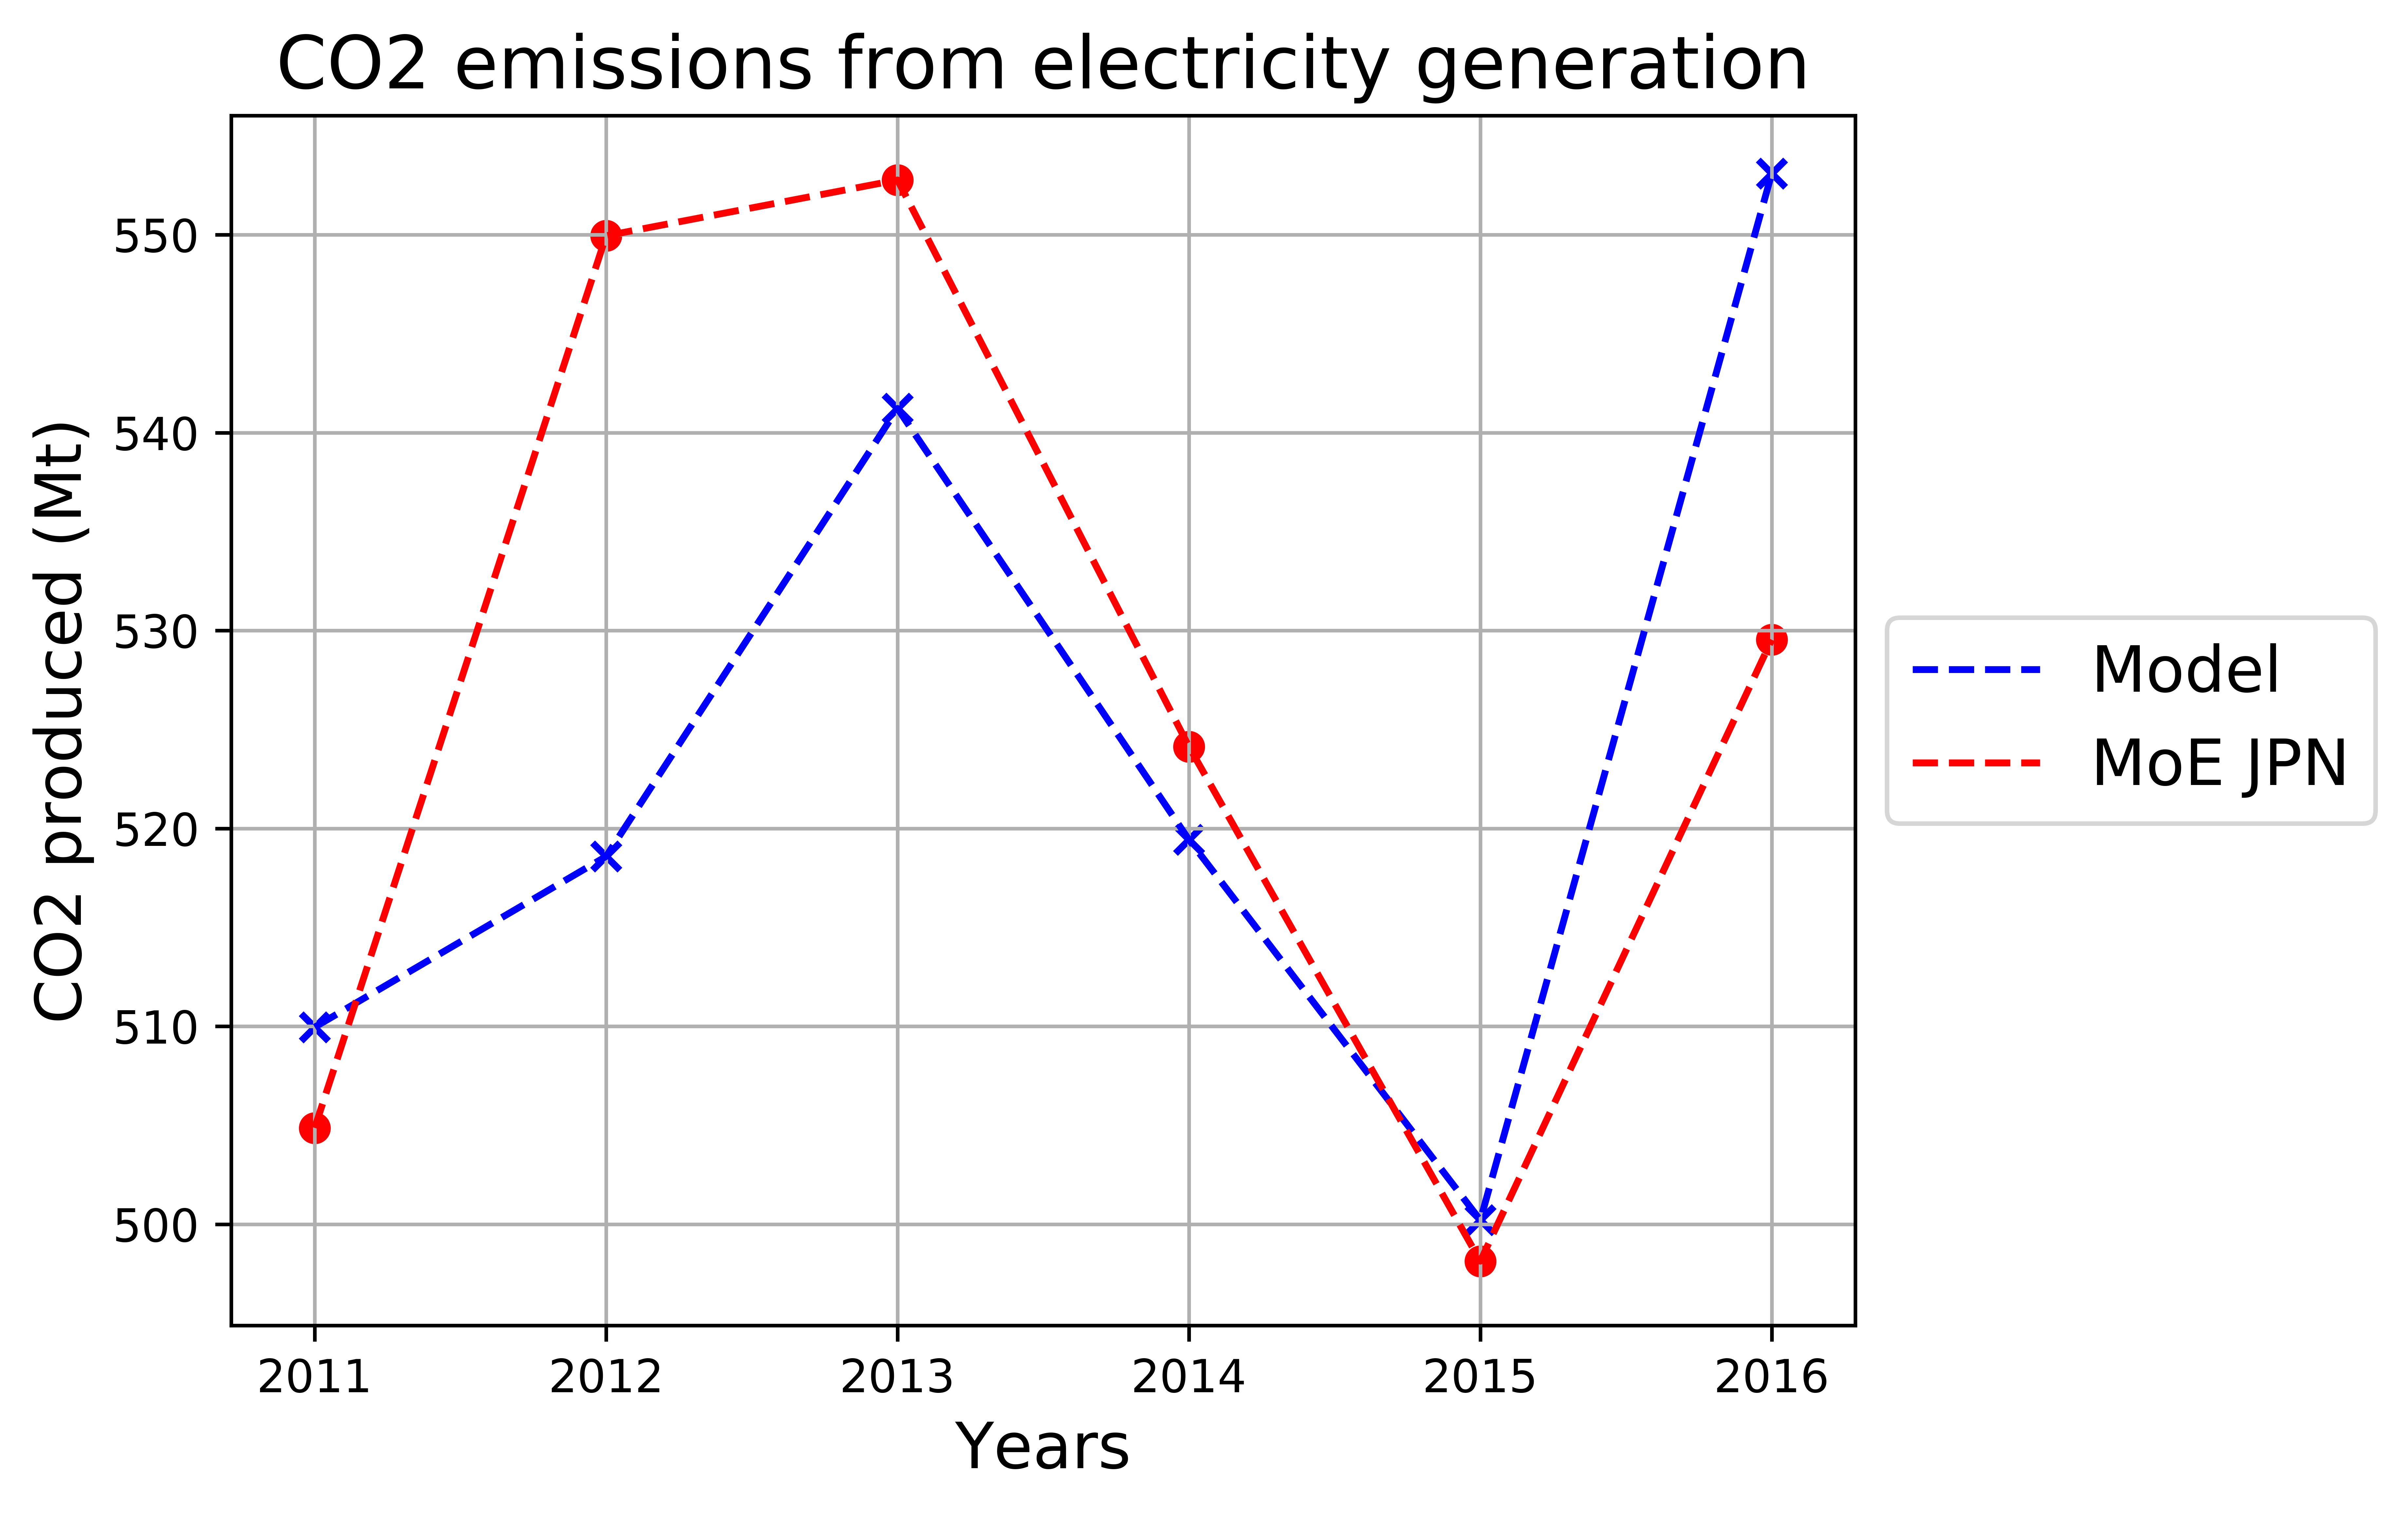
\includegraphics[scale=0.6]{co2-2016}
\caption{CO2 emissions from electricity generation compared with actual emissions reported by \gls{MOE}, Japan}
\label{co2ic}
\end{figure}

\begin{figure}[H] \label{co2err}
\centering
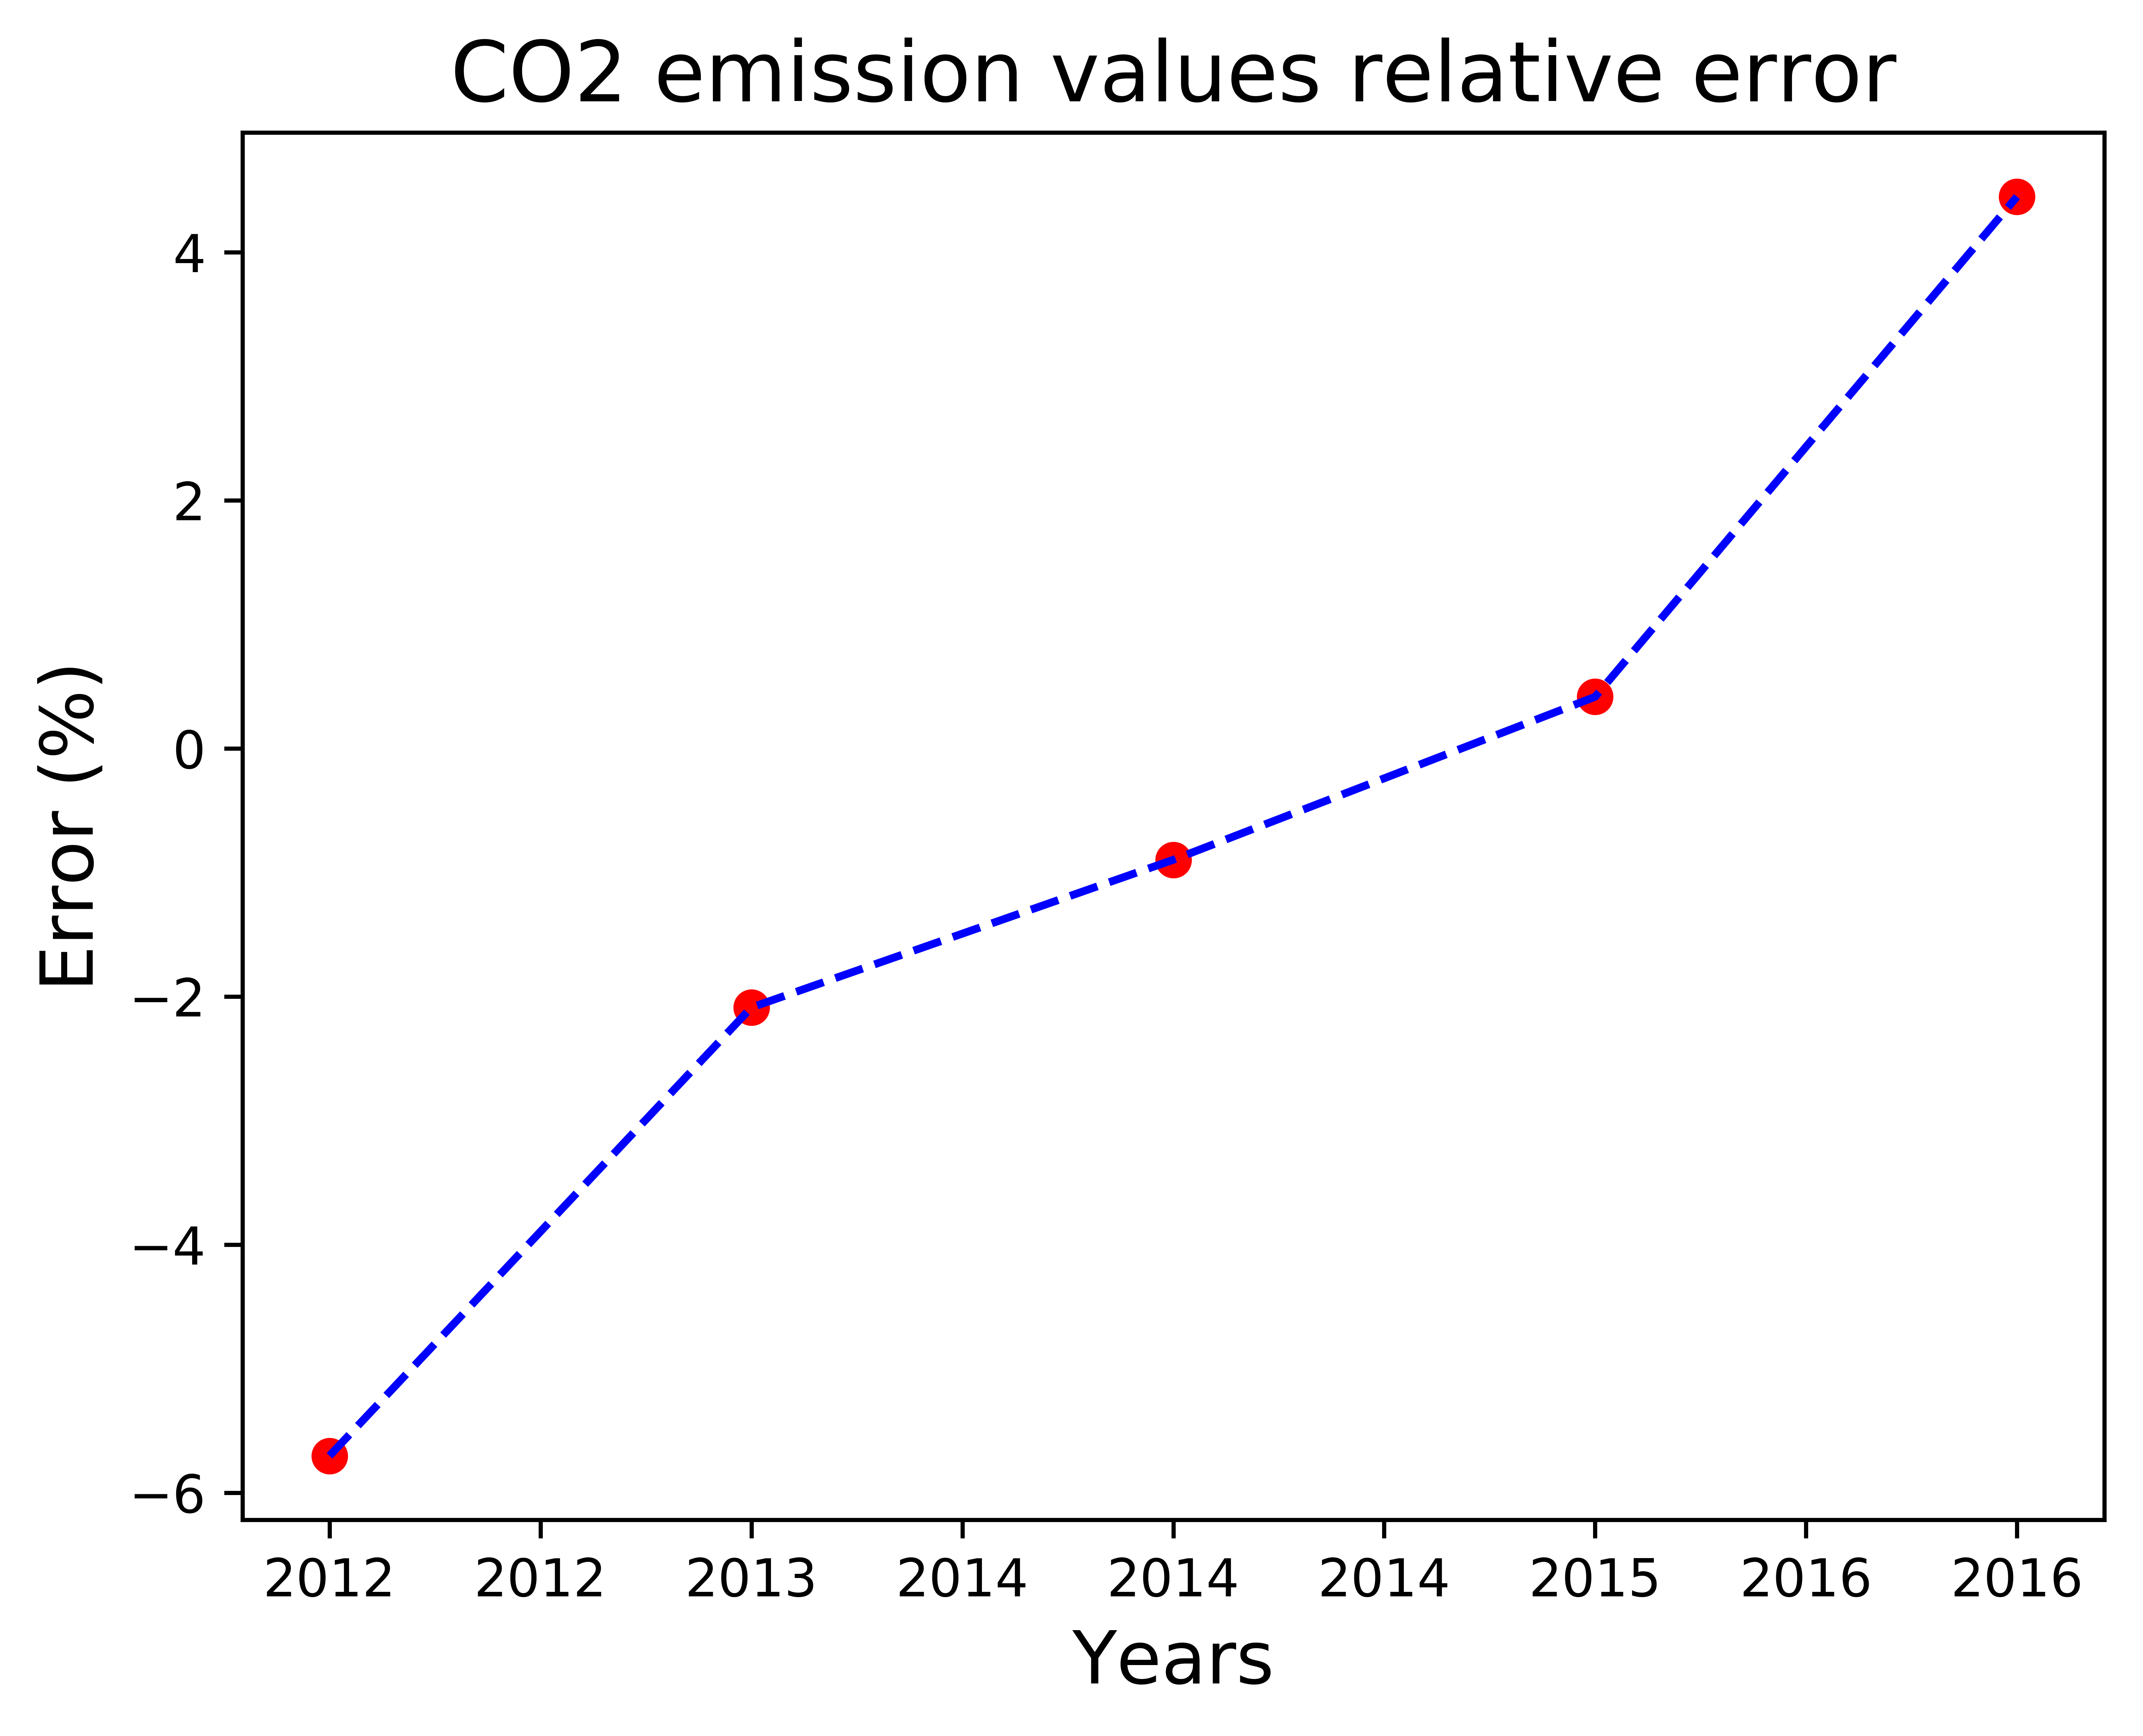
\includegraphics[scale=0.6]{co2-err}
\caption{Relative error in CO2 emissions.}
\label{co2err}
\end{figure}

As mentioned previously, the importance of incorporating semi-discrete installed capacity investment intervals is demonstrated by figures \ref{flatbug} and \ref{flatgood}. As seen in fig. \ref{flatbug}, production exceeds demand if semi-discrete investment intervals are not used in \gls{DSCINV} files. This issue is resolved if semi-discrete intervals are incorporated instead (see fig. \ref{flatgood}).

\begin{figure}[H]
\centering
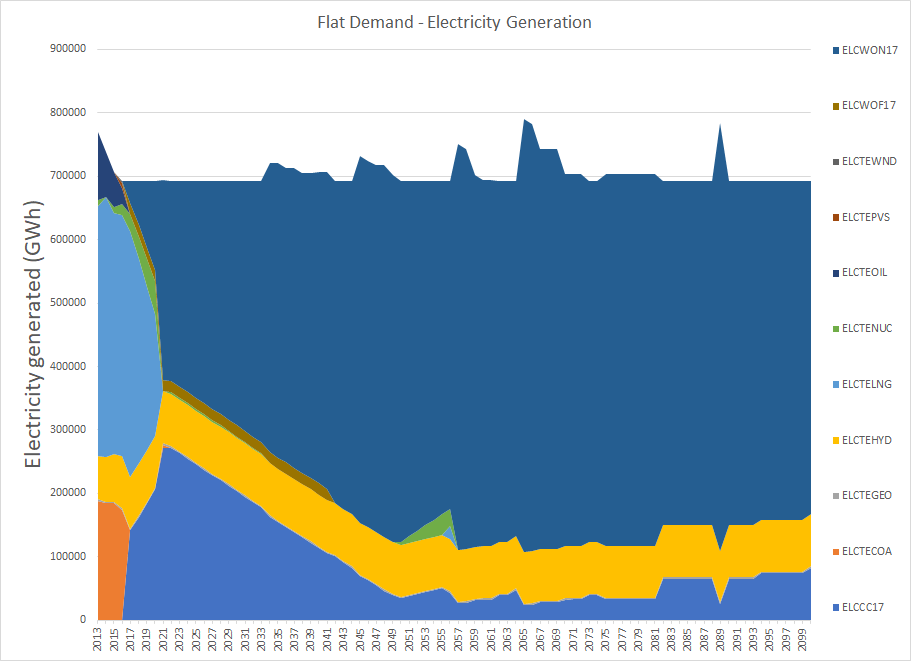
\includegraphics[scale=0.45]{flat-bug}
\caption{Erroneous results obtained with discrete investment sizes in \gls{DSCINV} files.}
\label{flatbug}
\end{figure}

\begin{figure}[H]
\centering
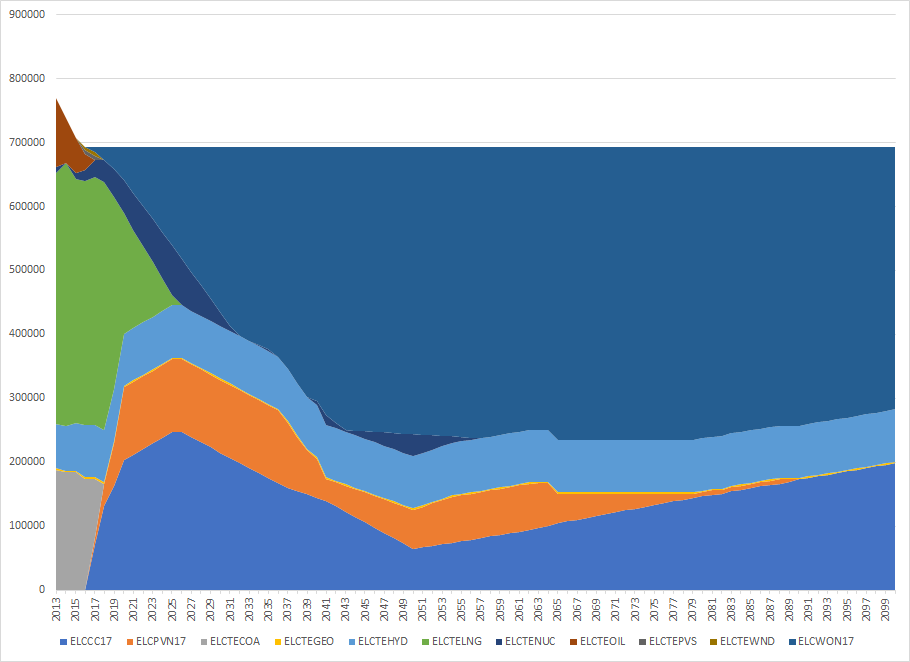
\includegraphics[scale=0.45]{flat-good}
\caption{Accurate results obtained with semi-discrete investment sizes in \gls{DSCINV} files.}
\label{flatgood}
\end{figure}

\subsection{Post Hoc Analysis and Challenges} 

The project has been delayed in part due to limited documentation and customer support available to VEDA users. The primitive, black-box like nature of the software inhibits efficient debugging. Therefore, while data acquisition and organization proceeded at the originally suggested pace, the incorporation of these data into the model has been behind schedule. \\

The \gls{EDMC} is constantly being revised and updated, for both earlier (2010-2013) and later years(2016-). Hence, these data are often inconsistent or incomplete, and hence secondary sources must be used for verification.
\section{Future Work} 

\subsection{Next Steps}

\textbf{Remove pure oil based electricity generation from all models:} We do not think Japan will ever increase its dependence on oil due to its cost, emissions intensity and due to the Japanese goal of increasing energy independence. Current trends support this assumption. While a few models already exclude oil-based energy, other models should also replace it with combined-cycle electricity generation for the sake of consistency.\\

\textbf{Incorporate semi-discrete investment sizes:} As stated previously, all \gls{DSCINV} files must include semi-discrete installed  capacity installation sizes for consistency.\\

\textbf{Restrict maximum wind installed  capacity:} To align the model more closely with JWPA predictions \cite{heger_wind_2016}, the maximum allowed capacities for wind should be reduced in the respective \gls{MaxCAP} files.\\

\textbf{Associate wind (and solar) with natural gas/storage:} There may be three ways to accomplish this:

\begin{itemize}

\item \textbf{Define load curves for solar and wind:} This is the approach suggested by VEDA developers on their forum. However, the details for implementation of this particular approach are lacking in the \gls{TIMES}/VEDA documentation. A successful implementation should incorporate the daily and seasonal variation of these electricity sources, and force the model to deploy natural gas or electricity storage to supplement wind and solar.

\item \textbf{Replace annually averaged  capacity factors and/or \gls{PEAK} factors with seasonal (summer/winter) and diurnal (day/night) (i.e. SN,SD, WN, WD \cite{gargiulo_documentation_2005}) capacity factors} : The model may then automatically deploy natural gas to supplement wind and solar. If seasonal versions of these factors exist, this would be the easiest solution. \gls{TIMES} Documentation Part II \cite{loulou_documentation_2005} may offer some insights in this regard.

\item \textbf{Define a direct relationship between the capacities of wind and natural gas}:It might be possible to define a direct equation between the installed  capacity of renewables and natural gas. Since no straightforward way to do this is described in the VEDA documentation \cite{gargiulo_documentation_2005}, this would require utilization of the \gls{TIMES} documentation \cite{loulou_documentation_2005}, the VEDA attributes table, and  possibly the assistance of the VEDA forum.

\end{itemize}

\textbf{Cost Analysis} - Some metric to compare the transition costs for each scenario should be calculated and presented with our results. For example, the \gls{LCOE} for each scenario for different years (say 2030,2050,2100) could be calculated, or the total cost of the transition (investment+generation) could be juxtaposed for each scenario.\\

\textbf{Incorporate more \gls{I2CNER} technology}, such as perovskite solar cells, fuel cells for storage etc.\\

\textbf{Sensitivity analysis:} To identify optimum thresholds for costs or parameters (like efficiency) of novel technologies, especially \gls{I2CNER} technology, to maximize their efficacy and penetration.\\

\subsection{Potential improvements}

\textbf{Revise \gls{CCS} costs:} Simplified \gls{CCS} electricity generation processes exist in our \gls{I2CNER} models. These emit only 10\% of the CO$_2$ that their corresponding fossil fuel technology emits \cite{kato_energy_2016}. In the model, these look like any other fossil fuel electricity generation process, except they are more expensive and have a significantly smaller emission coefficient. Such an implementation does \textbf{not} include retrofitting of \gls{CCS} (i.e. adding point carbon capture capabilities to previously deployed fossil fuel plants). While we do not have Japan-specific data for \gls{CCS}, we can use cost data from the US and do one of the following:

\begin{itemize}

\item Neglect the difference between Japan and the US, assuming that the government will foot the bill of setting up the \gls{CCS} shipping network and offshore storage sites.

\item Roughly increase the cost by a small percentage, since setting up the Japanese \gls{CCS} shipping network and offshore storage sites will result in an increased cost per unit CO$_2$ captured and stored.

\item Attempt to conduct a rough ab-initio analysis to find the cost of capturing, transporting and storing one ton of CO$_2$. The cost of capturing CO$_2$ is more or less uniform and readily available \cite{kato_energy_2016}. The cost of transport and storage can be estimated by finding the cost of offshore-drilling to the depths necessary for CO$_2$ storage, the cost of pressurizing 1 ton of CO$_2$, and the cost of transporting a ton of cargo to offshore storage sites by ship. The exact costs for this vary based on the scale of the operation.

\end{itemize}

\textbf{Replace \gls{LCOE} in all models with a detailed cost structure:} All models must incorporate investment and \gls{OM} costs.\\

\textbf{Incorporation of Japan-specific costs for wind:} When incorporating \gls{JWPA} predictions, it will be necessary to split off-shore wind into fixed and floating types. The \href{https://github.com/arfc/i2cner/tree/master/data/japan_costs}{cost data} for this already exist in our repository thanks to Akari Minami, an undergraduate from Kyushu University who assisted with data collection and simulation during March 2019. These data need to be sifted through and incorporated into our model.\\

\textbf{Revise nuclear costs:} Current models include the ideal cost of nuclear, but actual costs are often higher due to delays in construction. This is accurately reflected in data from \gls{EIA} \cite{noauthor_eia_2019}, which already exists in our \href{https://github.com/arfc/i2cner/tree/master/data/japan_costs/fossil-ccs-nuc.xlsx}{repository}. This needs to be incorporated into our models to reduce over-deployment of nuclear.\\

\paragraph{Make electricity demand process more realistic:} Demand should increase at +1.7 \% per year until 2030 as per \gls{METI} projections \cite{noauthor_electricity_2017}, and should plateau afterwards until 2100. More accurate data for 2030-2050 can be sought to further improve upon this, if possible.\\

\textbf{Implement \gls{CCS} retrofitting:} The modelling process for this is somewhat complicated. CO$_2$ emitted from different fossil fuels would have to be tracked separately by creating \gls{TIMES}  CO$_2$ commodities for coal, oil and petroleum, to ensure that CO$_2$ from non-fossil fuel sources is not captured by the model. Next, the process that converts this CO$_2$ to captured CO$_2$ and atmospheric CO$_2$ would need to be defined. The total amount of CO$_2$ captured should be less than the total capacity of the \gls{CCS} reservoirs around Japan \cite{kato_energy_2016}.\\
The data for retrofitting in Japan are not easily available. Generic \gls{CCS} data from other countries may be used if necessary.\\

\bibliographystyle{ieeetr}
%\addbibresource{2018-chaube-i2cner-report-sept}
\bibliography{2018-chaube-i2cner-report-sept}

%\bibliographystyle{plain}

%\printbibliography

\end{document}
